\documentclass[presentation]{beamer}
\usepackage{../oop-slides}

\title[OOP05: Incapsulamento]{05 \\ Incapsulamento}

\begin{document}

\newcommand{\ecl}{\idepath{p05encapsulation}}

\frame[label=coverpage]{\titlepage}

\fr{Outline}{
  \bl{Goal della lezione}{\iz{
  \item Illustrare concetti generali di incapsulamento e information hiding
  \item Mostrare tecniche di programmazione standard
  \item Fornire primi esempi di classi ben progettate
  }}
  \bl{Argomenti}{\iz{
  \item Convenzioni su formattazione
  \item Incapsulamento in Java
  \item Una metodologia di progettazione
  \item Ulteriori convenzioni
  
  }}
}


\fr{Ambiente integrato Visual Studio Code}{
  \bl{Funzionalità}{\iz{
  \item Supporto multi-linguaggio
  \item Vasta quantità di plug-in 
  \item Supporta editing ``intelligente'', compilazione on-the-fly, debug, esecuzione
  \item Concetto di progetto
  }}
  \bl{Metodologia}{\iz{
    \item creazione progetto, package, classi
    \item esecuzione dalla classe col main
    \item possibilità di importare/esportare file ZIP (p.e., codice aula)
  }}
}


\section{Alcuni principi di buona progettazione}

% Goal: avere criteri di progettazione che non solo permettano di arrivare alla soluzione del problema, ma anche permettere al risultato di essere facilmente mantenibile (spesso le due cose si assomigliano).. ossia se devo cambiare qualcosa ci metto poco e non mi rovina il resto
% Decomposizione (con basse interdipendenze, se vogliamo, separation of concern)
  % information hiding permette di calare le interdipendenze
    % encapsulation è il modo di risolvere la cosa nei ling OO
      % controllo d'accesso (mopdifiers)
      % impacchettamento di dati e funzioni (classe)
%--> Linee guida?

% Successivamente avremo composizione e riuso

\fr{Dai meccanismi alla buona progettazione/programmazione}{
  \bl{La nostra analisi dell'OO in Java finora, ci ha insegnato:}{\iz{
    \item Parte imperativa/procedurale di Java (tipi primitivi, operatori, cicli)
    \item Classi, oggetti, costruttori, campi, metodi
    \item Codice statico, controllo d'accesso
  }}
  \bl{Detto ciò, come realizziamo un buon sistema?}{
  Come programmiamo il sistema
  \en{
    \item per giungere al risultato voluto, e
    \item così che sia facilmente manutenibile (estendibile, flessibile, leggibile)?
  }}
  $\Rightarrow$ un percorso articolato: muoviamo i primi passi..
}

\fr{Passi}{
  \bl{Il nostro approccio}{
  \en{
    \item Ricapitoleremo le principali convenzioni sul codice Java 
    \item Anticiperemo alcune tecniche di programmazione efficace basate sulle tecniche di \alert{incapsulamento}, e conseguenti al fondamentale principio di \alert{decomposizione} ($\Leftarrow$ aspetto cruciale della OO)
    \item Daremo qualche linea guida utile in futuro per costruire sistemi di più grosse dimensioni
  }}
  \bx{Nota: tutte queste tecniche e linee guida sono necessarie per gestire il livello di articolazione del linguaggio Java, ossia per rendere il suo uso più semplice possibile}
}

\section{Convenzioni su formattazione}


\fr{Convenzioni sulla formattazione, pt 1}{
  \bl{Formattazione generale}{\iz{
    \item Indentazione di 2-4 caratteri (comunque non 1, non 10..)
    \item Linee lunghe non più di 90 caratteri -- spezzare in modo coerente
  }}
  \bl{Commenti nel codice}{\iz{
    \item ``\cil{// ...}'' su una linea
    \item ``\cil{/* ..*/}'' su più linee per commentare sezioni
    \item ``\cil{/**..*/}'' su più linee per commenti che generano documentazione
  }}
  \bl{Istruzioni}{\iz{
    \item Definizione di variabile: una per linea, solo quando/se serve
    \item Meglio inizializzare sempre le variabili!
    \item Una sola istruzione per riga 
  }}
}

\fr{Convenzioni sulla formattazione, pt 2}{
  \bl{Costrutti vari}{\iz{
    \item Apertura graffa: a fine linea della dichiarazione
    \item Chiusura graffa: in linea a sè, dove inizia la linea che la apre
    \item Metodi/costruttori separati da una linea vuota (poche separazioni altrimenti)
    \item Usare graffe anche con blocchi ad uno statement
    \item Non usare assegnamenti dentro a espressioni
    \item Disambiguare priorità non banali fra operatori, con parentesi
  }}
 \bl{Nomi}{\iz{
    \item Classi (e interface): iniziano con maiuscola
    \item Metodi, campi, variabili: iniziano con minuscola
    \item Se nome strutturato usare ``camelCasing''
    \item Campi costanti: tutte maiuscole con eventuale separatore ``\textunderscore''
  }}
}

\fr{Convenzioni sulla formattazione, pt 3}{
  \bl{Ordine delle proprietà della classe}{\iz{
    \item Campi statici (pubblici, poi privati)
    \item Campi istanza (pubblici, poi privati)
    \item Costruttori (pubblici, poi privati)
    \item Metodi (raggruppati per ruolo)
  }}
  \bl{Nota finale}{\iz{
    \item L'uso delle corrette convenzioni rende il codice molto più leggibile, ma anche a volte meno conciso
    \item Nelle slide è impossibile mostrarlo sempre in questo modo
    %\item Quindi talvolta alcune convenzioni non verranno usate nel
  }}
}

\fr{Esempio: Point3D pt 1}{
  \srcode{\tiny}{3}{32}{\ecl/Point3D.java}
}

\fr{Esempio: Point3D pt 2}{
  \srcode{\tiny}{34}{100}{\ecl/Point3D.java}
}

\section{Decomposizione, incapsulamento, information hiding}

\fr{Il principo di decomposizione}{
\bx{\Huge divide et impera}
\bl{Dividi e conquista: approccio \alert{top-down}}{\iz{
  \item La soluzione di un problema complesso avviene dividendolo in problemi più semplici, tra loro indipendenti
  \item La suddivisione è spesso multi-livello
}}
\bl{Esempi}{\iz{
\item SW calcolatrice con GUI: GUI, gestione eventi, calcoli matematici
\item Disegno Mandelbrot: Complex, Mandelbrot, MandelbrotApp
}}
}

\fr{Decomposizione, modularità e dipendenze}{
  \bl{Un punto cruciale della decomposizione è la ``modularità''}{\iz{
    \item La suddivisione va fatta in modo tale che sia effettivamente conveniente
    \item Bisogna isolare i ``sottoproblemi'' più semplici
    \item Ciò è possibile se riduciamo al massimo le ``dipendenze'' fra i sottoproblemi, il che consente:
    {\iz{
      \item più autonomia decisionale
      \item meno interazione con altri
      \item \alert{meno influenze negative nel caso di modifiche}
    }}
  }}
}

\fr{Modularità: quale situazione la preferibile?}{
\begin{center}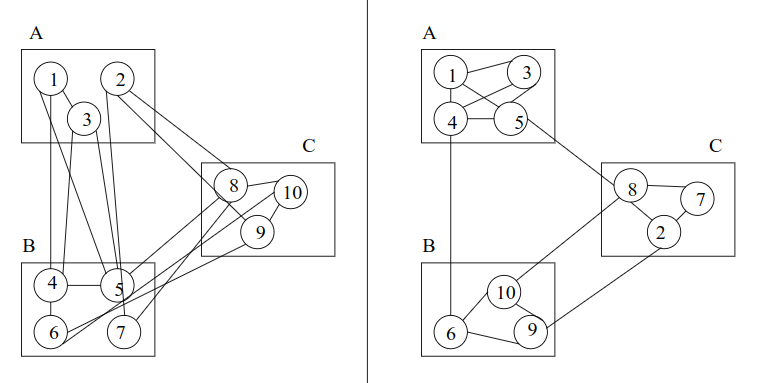
\includegraphics[height=0.6\textheight]{img/coupling.png}\end{center}
}


\fr{Decomposizione e programmazione OO}{
  \bl{Nella programmazione OO, almeno 3 livelli di decomposizione}{\en{
    \item Suddivisione in package (dell'intero programma)
    \item Suddivisione in classi (di un package o programma)
    \item Suddivisione in metodi (di una classe)
  }}
  \bl{La OOP affronta principalmente la suddivisone in classi}{\iz{
    \item È necessario suddividire il codice in classi nel modo opportuno
    \item Creando il miglior link col ``problem space''
    \item \alert{Diminuendo il più possibile le dipendenze fra classi}
  }}
  \bl{Tecnica}{\iz{
    \item Esistono consolidate pratiche di programmazione efficace che risolvono il problema, e che cominceremo ad analizzare in questa lezione -- farlo bene richiede significativa esperienza!
  }}
}

\fr{Dipendenze e OO}{
  \bl{Dipendenza}{
    Si dice che una classe \cil{A} dipende da una classe \cil{B} se all'interno del codice di \cil{A} si menziona la classe \cil{B} (ad esempio come input di un metodo) o qualche suo mmebro. La dipendenza è tanto più profonda quanto più in \cil{A} si usano anche costruttori e/o campi e/o metodi definiti in \cil{B}.
  }
  \bl{Implicazione}{
    Ogni dipendenza vincola fortemente la possibilità di fare modifiche, perché ne comporta altre da fare in cascata. Se \cil{A} dipende da \cil{B} e modifico \cil{B}, dovrò probabilmente modificare anche \cil{A}.
  }
  \bl{La sindrome dell'``intoccabilità''---SW rigido}{
    Costruendo software complesso con troppe dipendenze, si giunge al punto che ogni singola modifica ne richiederebbe molte altre, e rischierebbe quindi di essere troppo costosa -- risultato: non si cambia più il software!
  }
}

\fr{Incapsulamento}{
  \bl{Due ingredienti cruciali della programmazione OO}{\en{
    \item Impacchettamento dati + funzioni per manipolarli
    \item Information hiding via controllo d'accesso
  }}
  \bl{Filosofia}{\iz{
    \item Ogni classe dichiari \cil{public} solo quei (pochi) metodi/costruttori necessari a interagire con (o creare) le sue istanze
    \item Il resto (che quindi include meri aspetti realizzativi) sia \cil{private}{\iz{
      \item metodi/costruttori a solo uso interno
      \item {\bf{tutti}} i campi (ossia lo stato interno)
    }}
  }}
  \bl{Incapsulamento e dipendenze}{Così facendo il ``cliente'' è debolmente influenzato da possibili modifiche future riguardanti aspetti realizzativi e non di ``design''.
  }
}

\fr{Esempio base: Classe Counter}{
  \srcode{\footnotesize}{3}{32}{\ecl/Counter.java}
}

\fr{Semplice uso}{
  \srcode{\footnotesize}{3}{32}{\ecl/UseCounter.java}
}


\frs{5}{Uso contatore}{
  \bl{La classe contatore}{\iz{
   \item Incapsula una semplice funzionalità di conteggio
   \item Dà un approccio più astratto rispetto all'uso diretto di un \cil{int}
   \item Consende di agire sul conteggio solo con \cil{getValue()} e \cil{increment()}
   \item[$\Rightarrow$] è impossibile modificare il conteggio a piacimento (o per errore), ad esempio decrementando invece che incrementando, o azzerando
   \item[$\Rightarrow$] nota, il codice qui sotto è più astratto, ossia più di alto livello: non sono presenti operazioni matematiche esplicite!
  }}
   \srcode{\footnotesize}{5}{14}{\ecl/UseCounter2.java}
}

\fr{Uso contatore, pt 2}{
  \bl{Altra possibilità}{\iz{
    \item Passo il contatore alle funzioni che hanno bisogno di conteggi
    \item Ciò consente un più ampio grado di riuso
    \item In generale, sisono aperte nuove possibilità di riuso
  }}
  \srcode{\scriptsize}{16}{30}{\ecl/UseCounter2.java}
}

\fr{Riflessione: incapsulazione e contratto}{
  \bl{Contratto}{\iz{
    \item Il contratto di un oggetto corrisponde ai suoi scenari di utilizzo
    \item E quindi alle aspettative che un cliente ha quando usa l'oggetto
    \item Grazie all'incapsulamento, è possibile vincolare fortemente questi contratti, controllando meglio il comportamento degli oggetti
  }}
  \bl{Il caso del Contatore}{\iz{
    \item Il valore del conteggio all'atto della costruzione è \cil{0}
    \item Il valore del conteggio in ogni altro istante è pari al numero di chiamate di \cil{increment()}
  }}
  \bl{Osservazione}{
    \`E grazie a questa idea che è più facile comporre oggetti in sistemi più complicati (vedi funzione \cil{countInMatrix})
  }
}

\frs{13}{Oggetti immutabili}{
  \bl{Cosa sono}{\iz{
    \item Oggetti per i quali è garantito che il valore iniziale dei campi non si modificherà mai
    \item Portano un ulteriore livello di indipendenza (e semplicità/eleganza) nel codice
    \item In alcuni casi potrebbero portare a soluzioni poco performanti
  }}
  \bl{Come si costruiscono}{\iz{
    \item I campi della classe sono dichiarati \cil{final} (oltre che \cil{private}), e..
    \item ..contengono a loro volta valori primitivi o oggetti immutabili
    \item Quindi nessun metodo può modificarli (solo i costruttori possono, la prima volta)
    \item Invece che cambiare i campi si possono solo creare oggetti con nuovo stato
  }}
  \bl{Osservazione}{
    Per ora è sufficiente saperli riconoscere e costruire
  }
  \bl{Favorire sempre immutabilità ove possibile -- un principio avanzato}{
    Indicare anche \cil{final} variabili e argomenti che non verranno modificati
  }
}

\fr{\Cil{ImmutablePoint3D}}{
  \srcode{\tiny}{3}{100}{\ecl/immutable/ImmutablePoint3D.java}
}

\fr{\Cil{UseImmutablePoint3D}}{
  \srcode{\ssmall}{3}{100}{\ecl/immutable/UseImmutablePoint3D.java}
}

\section{Una metodologia basata sull'incapsulamento}

\fr{Altro esempio: classe \Cil{Lamp}}{
  \bl{Analisi del problema}{
    In un sistema domotico, dovremo gestire un certo numero di lampadine (da accendere/spegnere e pilotare tramite un apposito controllore centralizzato, oltre che tramite i comandi a muro). Tali comandi sono a pulsante, dotato anche di controllo di intensità ``dimmer'' (10 livelli). Il controllore deve poter accedere alla situazione di ogni lampadina (accesa/spenta, livello di intensità) e modificarla a piacimento. Al primo avvio, le lampadine sono spente e il controllo di intensità è a zero (in un intervallo $[0,1]$).
  }
  \bx{Come procediamo alla costruzione della classe \cil{Lamp}?}
}

\fr{Progettazione e implementazione: fasi}{
  \bl{Fasi nella costruzione di una classe}{\en{
    \item Progettazione della parte pubblica della classe
    \item Costruzione dello stato
    \item Completamento implementazione
    \item Miglioramento codice finale
    \item Test del risultato
  }}
  (negli approcci moderni si testa anche tra la fase 3 e 4)
}

\fr{Fase 1: Progettazione della parte pubblica della classe}{
  \bx{Ovvero, del nome della classe e delle signature di operazioni pubbliche (metodi e costruttori)}
  \bl{Linee guida}{\iz{
    \item Considerare tutti i vari casi d'uso di un oggetto della classe
    \item Inserire costruttori e metodi pubblici solo per le operazioni necessarie
    \item Evitare ove possibile di inserire un numero elevato di tali operazioni
  }}
  \bl{Il caso \cil{Lamp}}{\iz{
    \item Un costruttore unico senza argomenti
    \item Metodi per accendere/spegnere
    \item Metodi per aumentare/ridurre/impostare intensità
    \item Metodi per accedere allo stato della lampadina
  }}
  
}

\fr{Parte pubblica della classe \Cil{Lamp}}{
  \sizedcode{\footnotesize}{code/IntLamp.java}
}


\fr{Fase 2: Costruzione dello stato}{
  \bx{Ovvero, dei campi privati della classe}
  \bl{Linee guida}{\iz{
    \item Considerare che esistono varie scelte possibili (è un aspetto implementativo, ritrattabile successivamente)
    \item L'insieme dei campi deve essere più piccolo possibile, per esigenze di performance (spazio in memoria) e di non duplicazione
    \item L'insieme dei campi deve essere sufficiente a tenere traccia di tutti i modi in cui il comportamento dell'oggetto può cambiare a fronte dei messaggi ricevuti
  }}
  \bl{Il caso \cil{Lamp}}{\iz{
    \item Dovremo sapere se è accesa o spenta (\cil{boolean switchedOn})
    \item Dovremo sapere il livello attuale di intensità (\cil{double intensity})
    \item Non sembrano servire altre informazioni
  }}
}

\fr{Stato e metodi della classe \Cil{Lamp}}{
  \code{code/FieLamp.java}
}


\fr{Fase 3: Completamento implementazione}{
\bx{Ovvero, del corpo di costruttori e metodi}
  \bl{Linee guida}{\iz{
    \item Realizzare il corpo di ogni costruttore e metodo in modo compatibile col contratto previsto per la classe
    \item Accettare il fatto che la prima versione prodotta non necessariamente sarà quella finale
  }}
  \bl{Il caso \cil{Lamp}}{\iz{
    \item \cil{switchOn()}, \cil{switchOff()} sono semplici \alert{setter} del campo \cil{switchedOn}
    \item \cil{isSwitchedOn()}, \cil{getIntensity()} semplici \alert{getter} dei due campi
    \item \cil{dim()} e \cil{brigthen()} modificano il campo \cil{intensity} (se nel range!)
  }}
}

\fr{Prima versione Classe Lamp}{
  \sizedcode{\tiny}{code/Lamp1.java}
}

\fr{Fase 4: Miglioramento codice finale}{
  \bl{Linee guida}{\iz{
    \item Inserire commenti nel codice
    \item Verificare la necessità di costanti per evitare numeri ``magici''
    \item Eventualmente fattorizzare sotto-funzioni in metodi/costruttori pubblici/privati, per evitare duplicazioni
  }}
  \bl{In concreto in questo caso}{\iz{
    \item Vi sono numeri magici, usare costanti!
    \item Gestire meglio il limite $0..1$
    \item Evitare livelli intermedi ($0.145$) di luminosità
    \item Ritrattare la scelta del tipo del campo \cil{intensity} -- meglio un \cil{int} fra $0$ e $10$!!
    \item \alert{Grazie all'incapsulamento possiamo cambiare i campi senza modificare i client!}
  }}
}

\fr{Versione finale Classe Lamp -- A}{
  \srcode{\ssmall}{3}{30}{\ecl/Lamp.java}
}

\fr{Versione finale Classe Lamp -- B}{
  \srcode{\ssmall}{32}{100}{\ecl/Lamp.java}
}


\fr{Fase 5: Test del risultato}{
  \bl{Linee guida}{\iz{
    \item Definire un insieme di scenari d'uso di un oggetto
    \item Per ognuno costruire una procedura che crea l'oggetto, lo usa, e stampa i risultati necessari
  }}
  \bl{Il caso \cil{Lamp}}{Un possibile caso (non costituisce da solo un test esaustivo):\iz{
    \item Costruisco l'oggetto lampadina
    \item La accendo
    \item Imposto la luminosità, poi la vario un poco
    \item Leggo e stampo lo stato del sistema
  }}
}

\fr{Classe UseLamp}{
  \srcode{\footnotesize}{3}{30}{\ecl/UseLamp.java}
  %\sizedcode{\footnotesize}{code/classes/UseLamp.java}
}

\fr{Il metodo toString()}{
  \bl{Una convenzione Java}{\iz{
    \item Ogni classe dovrebbe definire un metodo \cil{toString()}
    \item Questo deve restituire una rappresentazione in stringa dell'oggetto
    \item Così si incapsula anche la funzionalità di presentazione (su console)
    \item Tale metodo è quello che viene automaticamente chiamato quando si usa l'operatore \cil{+} per concatenare stringhe a oggetti
  }}
}

\fr{UseLamp: uso di toString}{
  
  \sizedcode{\scriptsize}{code/classes/UseLampString.txt}
}

\fr{Il collaudo di Lamp è completato?}{
  \bl{Quanti scenari di test vanno preparati?}{\iz{
    \item Non c'è un numero giusto
    \item Non è possibile in generale controllare in modo completo
    \item Bisogna trovare il giusto rapporto tempo/risultato
    \item Certamente, un unico scenario è insufficiente
    \item La metodologia ``test-driven development'' consiglia di costruire test esaustivi prima dell'effettivo sviluppo di ogni funzionalità{\iz{
	\item Inizialmente percepito come un po' noioso
	\item Sembra far perdere tempo
	\item Spesso ripaga in termini di temi complessivi e qualità del software profotto
	\item Vedremo framework dedicati ai test (\cil{JUnit})
    }}
  }}
}



\section{Ulteriori convenzioni e linee guida}

\fr{Convenzione Java sui nomi di metodi getter/setter}{
  \bl{Metodi getter/setter}{\iz{
    \item Un metodo \alert{getter} è un metodo che senza input restituisce un valore, una proprietà dell'oggetto
    \item Un metodo \alert{setter} è un metodo che restituisce \cil{void} e accetta un valore che modifica una proprietà dell'oggetto
    \item (Tali proprietà sono spesso campi, ma ciò non è necessario)
    \item In \cil{Lamp}, \cil{getIntensity} e \cil{isSwitchedOn} sono getter, \cil{setIntensity} è un setter
  }}
  \bl{Convenzione sul nome del metodo: sia data la proprietà \cil{XYZ} di tipo \cil{T}}{\iz{
    \item Getter non booleano: \cil{T getXYZ()\{...\}}
    \item Getter booleano: \cil{boolean isXYZ()\{...\}}
    \item Setter: \cil{void setXYZ(T xYZ)\{...\}}
  }}
}

\fr{Getter/setter in Lamp}{
  \sizedcode{\ssmall}{code/LampGS.java}
}



\end{document}

\fr{LampUtilities}{
  \srcode{\tiny}{3}{30}{\ecl/LampUtilities.java}
}


\fr{Altro esempio di buon incapsulamento e immutabilità}{
  \bl{\cil{MandelbrotApp}}{\iz{
    \item Trovate nel materiale fornito una versione ben incapsulata dell'applicazione che disegna il set di Mandelbrot
  }}
  \bl{Principali differenze}{\iz{
    \item campi sempre privati (se usati da altri diventano metodi ``getter''
    \item altre proprietà (costanti o metodi) pubbliche o private se usate o meno da fuori
  }}
}


\fr{Sull'uso di codice statico}{
  \bl{Codice statico}{\iz{
    \item Metodi statici: funzionalità relative alla classe ma che non si associano ad un oggetto specifico
    \item Campi statici: variabili relative alla classe ma che non si associano ad un oggetto specifico
    \item Inizializzatore statico: codice di inizializzazione per campi statici
  }}
  \bl{Raccomandazioni}{\iz{
    \item L'uso di codice statico e non-statico (istanza) in una stessa classe è considerato troppo sofisticato, e di difficile lettura
    \item \`E buona prassi di programmazione cercare di non mischiarli {\iz{
      \item Nelle librerie Java, tuttavia, non si usa questa raccomandazione
    }}
    \item Laddove serva codice statico, si usi una classe a sé che lo contenga
    \item Si tollera solo l'uso di costanti (campi \cil{static final})
  }}
}
